% Dit werk is gelicenseerd onder de licentie Creative Commons Naamsvermelding-GelijkDelen 4.0 Internationaal. Ga naar http://creativecommons.org/licenses/by-sa/4.0/ om een kopie van de licentie te kunnen lezen.
\documentclass[t]{beamer}

\usepackage{amsmath,amsthm}             % Uitgebreide wiskundige mogelijkheden
\usepackage{xcolor}						% Om kleuren te gebruiken

%%%%%%%%%%%%%%%%%%%%%%%%%%%%%%%%%%%%%%%%%%%%%%%%%%%%%%%%%%%%
% Nieuwe commandos
%%%%%%%%%%%%%%%%%%%%%%%%%%%%%%%%%%%%%%%%%%%%%%%%%%%%%%%%%%%%

% De differentiaal operator
\newcommand{\diff}{\ensuremath{\mathrm{d}}}
\newcommand{\subsdiff}{\ensuremath{\mathrm{D}}}
\newcommand{\vardiff}{\ensuremath{\mathrm{\delta}}}

% Super en subscript
\newcommand{\supsc}[1]{\ensuremath{^{\text{#1}}}}   % Superscript in tekst
\newcommand{\subsc}[1]{\ensuremath{_{\text{#1}}}}   % Subscript in tekst

% Vectoren en matrices
\newcommand{\vt}[1]{\ensuremath{\boldsymbol{#1}}} % vector in juiste lettertype
\newcommand{\mx}[1]{\ensuremath{\mathsf{#1}}}	  % matrix in juiste lettertype

% Nieuw commando om iets te benadrukken en tegelijkertijd in de index te steken.
\newcommand{\begrip}[1]{\index{#1}\textbf{#1}\xspace}

% Graden celcius
\newcommand{\degC}{\ensuremath{^\circ \mathrm{C}}}
% graden
\renewcommand{\deg}{\ensuremath{^\circ}}

% unit
\newcommand{\unit}[1]{\ensuremath{\mathrm {#1}}}


% underlinered
\newcommand{\underlinered}[1]{\color{red}\underline{{\color{black}#1}}\color{black}}
%%%%%%%%%%%%%%%%%%%%%%%%%%%%%%
% Packages
%%%%%%%%%%%%%%%%%%%%%%%%%%%%%%

%\usepackage{geometry}              	% 
\usepackage[dutch]{babel}               % Voor nederlandstalige hyphenatie (woordsplitsing)
\uselanguage{dutch}
\languagepath{dutch}
\usepackage{amsmath,amsthm}             % Uitgebreide wiskundige mogelijkheden
\usepackage{url}                        % Om url's te verwerken
\usepackage{graphicx,subfigure}         % Om figuren te kunnen verwerken
\usepackage[utf8]{inputenc}             % Om niet ascii karakters rechtstreeks te kunnen typen
\usepackage[section]{placeins}			% Om ervoor te zorgen dat floats binnen dezelfde section blijven
\usepackage{multicol}
\usepackage[absolute,overlay]{textpos}

%%%%%%%%%%%%%%%%%%%%%%%%%%%%%%
% Layout
%%%%%%%%%%%%%%%%%%%%%%%%%%%%%%
\usetheme{Frankfurt}
\usefonttheme[onlymath]{serif}
\AtBeginSection[]
{
  \begin{frame}
    \frametitle{Inhoud}
    \tableofcontents[currentsection]
  \end{frame}
}

\setbeamertemplate{navigation symbols}{}
\setbeamertemplate{footline}[page number]

%%%%%%%%%%%%%%%%%%%%%%%%%%%%%%
% Title
%%%%%%%%%%%%%%%%%%%%%%%%%%%%%%
\title{Fluïdummechanica}
\author{Brecht Baeten\inst{1}}
\institute{
	\inst{1}%
  		KU Leuven, Technologie campus Diepenbeek,\\ e-mail: brecht.baeten@kuleuven.be
}
\date{\today}
%%%%%%%%%%%%%%%%%%%%%%%%%%%%%%
% Omgevingen
%%%%%%%%%%%%%%%%%%%%%%%%%%%%%%


\subtitle{Stroming in leidingen}

\begin{document}

	\frame{\titlepage}
%%%%%%%%%%%%%%%%%%%%%%%%%%%%%%%%%%%%%%%%%%%%%%%%%%%%%%%%%%%%%%%%%%%%%%%%%%%
	\section{Inleiding}
	\begin{frame}
		\frametitle{Voorbeeld}
		\center
    	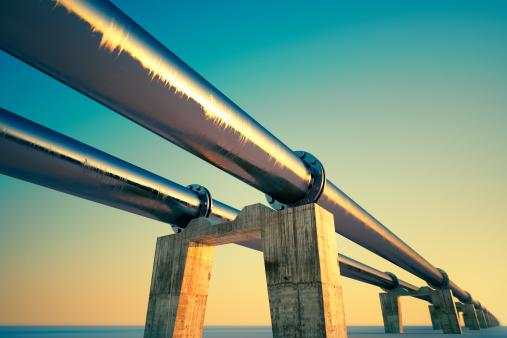
\includegraphics[width=\textwidth]{../fig/stroming_in_leidingen/Richard-Steinberg-The-Pipeline-Blog-51.jpg}\\
    	\footnotesize{Bron: http://www.etftrends.com/}
  	\end{frame}
  	\begin{frame}
  		\frametitle{Ontwikkelende stroming}
  		\center
  		\vspace{1.5cm}
  		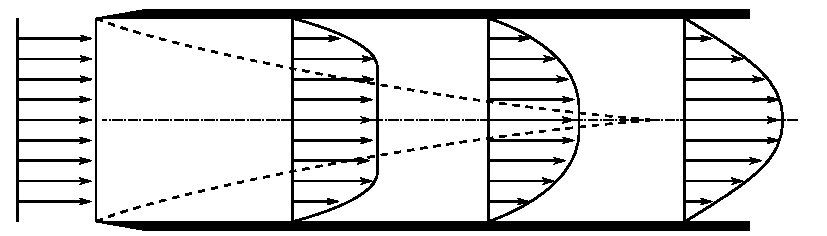
\includegraphics[width=\textwidth]{../fig/stroming_in_leidingen/Ontwikkelende_stroming}
  	\end{frame}	
%%%%%%%%%%%%%%%%%%%%%%%%%%%%%%%%%%%%%%%%%%%%%%%%%%%%%%%%%%%%%%%%%%%%%%%%%%%
  	\section{Dimensieanalyse}
  	\begin{frame}
		\frametitle{Dimensieanalyse}
		\begin{equation*}
			\Delta p = \phi(L,D,v,\mu,\rho)
		\end{equation*}
		\pause
		
		Buckingham Pi, ($n=5$,$k=3$)
		
		\pause
		\begin{equation*}
			\frac{\Delta p}{\frac{1}{2}\rho v^2} = f(L/D,Re)
		\end{equation*}
		\pause
		\begin{equation*}
			\frac{\Delta p}{\frac{1}{2}\rho v^2} = f(Re) \frac{L}{D}
		\end{equation*}
		\pause
		
		\begin{equation}
			\Delta p = f(Re) \frac{1}{2}\rho v^2 \frac{L}{D}
		\end{equation}
	\end{frame}
%%%%%%%%%%%%%%%%%%%%%%%%%%%%%%%%%%%%%%%%%%%%%%%%%%%%%%%%%%%%%%%%%%%%%%%%%%%
  	\section{Laminaire stroming}
  	\begin{frame}
		\frametitle{Snelheidsprofiel}
		\only<1>{
			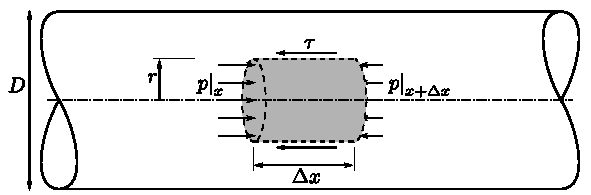
\includegraphics[width=\textwidth]{../fig/stroming_in_leidingen/Laminaire_stroming_in_buis}
		}
		\only<2-9>{
			\begin{textblock}{5}(0,3)
            	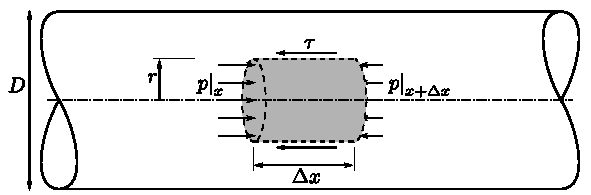
\includegraphics[width=5cm]{../fig/stroming_in_leidingen/Laminaire_stroming_in_buis}
       		\end{textblock}
       		\vspace{2cm}
		}
		\only<2-5>{
			Behoud van impuls in de stromingsrichting:
			\begin{equation*}
				F_x = 0
			\end{equation*}
		}
		\only<3-5>{
			\vspace{-0.5cm}
			\begin{equation*}
				\left. p \pi r^2\right|_{x} - \left. p \pi r^2\right|_{x+\Delta x} -  \tau 2 \pi r \Delta x = 0
			\end{equation*}
		}
		\only<4-5>{
			\begin{equation*}
				-\frac{1}{2} \frac{\diff p}{\diff x} r= \tau
			\end{equation*}
		}
		\only<5-5>{
			Newtoniaanse vloeistof:
			\begin{equation*}
				\frac{1}{2} \frac{\diff p}{\diff x} r = \mu \frac{\diff v}{\diff r}
			\end{equation*}
		}
		\only<6-9>{
			\begin{equation*}
				\frac{\diff v}{\diff r} = \frac{1}{2 \mu}\frac{\diff p}{\diff x} r
			\end{equation*}
		}
		\only<7-9>{
			\begin{equation*}
				v = \frac{1}{4 \mu}\frac{\diff p}{\diff x} r^2 + C
			\end{equation*}
		}
		\only<8-9>{
			\hspace{5cm} $\Downarrow \quad \begin{array}{rcl} \left.v\right|_{r=R} &=& 0 \\ C &=& - \dfrac{1}{4 \mu}\dfrac{\diff p}{\diff x} R^2\end{array}$ 
		}
		\only<9-9>{
			\begin{equation}
				v = - \frac{1}{4 \mu}\frac{\diff p}{\diff x} R^2 \left(1- \frac{r^2}{R^2}\right)
			\end{equation}
		}
		\only<10-11>{
			\begin{equation*}
				\frac{v}{v_\mathrm{max}} = \left(1- \frac{r^2}{R^2}\right)
			\end{equation*}
			\begin{equation*}
				v_\mathrm{max} = - \frac{1}{4 \mu}\frac{\diff p}{\diff x} R^2
			\end{equation*}
		}
		\only<11-11>{
			
			\vspace{0.5cm}
			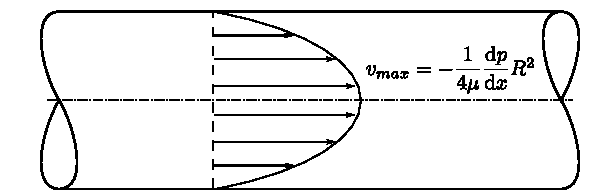
\includegraphics[width=\textwidth]{../fig/stroming_in_leidingen/Laminair_snelheidsprofiel}
		}
	\end{frame}
%%%%%%%%%%%%%%%%%%%%%%%%%%%%%%%%%%%%%%%%%%%%%%%%%%%%%%%%%%%%%%%%%%%%%%%%%%%
  	\begin{frame}
		\frametitle{Gemiddelde snelheid}
		\only<1-2>{
			\begin{textblock}{5}(0,3)
            	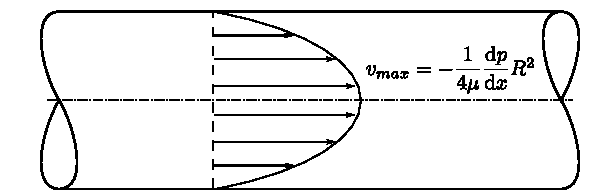
\includegraphics[width=5cm]{../fig/stroming_in_leidingen/Laminair_snelheidsprofiel}
       		\end{textblock}
       		\vspace{2cm}
		}
		\only<1-2>{
			Debiet:
			\begin{equation*}
				\dot{V} = 2 \pi \int_0^R v_\mathrm{max} \left(1- \frac{r^2}{R^2}\right) r \diff r = v_\mathrm{max} \frac{\pi R^2}{2}
			\end{equation*}
		}
		\only<2-2>{
			Gemiddelde snelheid:
			\begin{equation}
				v_\mathrm{gem} = \frac{\dot{V}}{\pi R^2} = \frac{v_\mathrm{max}}{2} = - \frac{1}{8 \mu}\frac{\diff p}{\diff x} R^2
			\end{equation}
		}
	\end{frame}
%%%%%%%%%%%%%%%%%%%%%%%%%%%%%%%%%%%%%%%%%%%%%%%%%%%%%%%%%%%%%%%%%%%%%%%%%%%
  	\begin{frame}
		\frametitle{Drukval}
		\only<1-5>{
			\begin{equation*}
				v_\mathrm{gem} = - \frac{1}{8 \mu}\frac{\diff p}{\diff x} R^2
			\end{equation*}
		}
		\only<2-5>{
			\begin{equation*}
				\frac{\diff p}{\diff x} = - 8 \mu v_\mathrm{gem} \frac{1}{R^2}
			\end{equation*}
		}
		\only<3-5>{
			\hspace{5cm} $\Downarrow \quad  \begin{array}{rcl} \dfrac{\diff p}{\diff x} &=& -\dfrac{\Delta p}{L}\\ R &=& D/2 \end{array}$
		}
		\only<4-5>{
			\begin{equation*}
				\Delta p = 32 \mu v_\mathrm{gem} \frac{L}{D^2}
			\end{equation*}
		}
		\only<5-5>{
			\begin{equation*}
				\Delta p = \frac{1}{2} \rho v^2 \frac{64 \mu}{\rho v D} \frac{L}{D}
			\end{equation*}
		}
		\only<6-9>{
			\begin{equation*}
				\Delta p = \frac{1}{2} \rho v^2 \frac{64 \mu}{\rho v D} \frac{L}{D}
			\end{equation*}
		}
		\only<7-9>{
			\begin{equation*}
				\Delta p = \frac{1}{2} \rho v^2 \frac{64}{\mathrm{Re}} \frac{L}{D}
			\end{equation*}
		}
		\only<8-9>{
			\vspace{0.5cm}
			\begin{equation}
				\Delta p = \frac{1}{2} \rho v^2 f \frac{L}{D}
			\end{equation}
		}
		\only<9-9>{
			\vspace{0.5cm}
			\center
			wrijvingsfactor voor laminaire stroming $f = \dfrac{64}{\mathrm{Re}}$
		}
	\end{frame}
%%%%%%%%%%%%%%%%%%%%%%%%%%%%%%%%%%%%%%%%%%%%%%%%%%%%%%%%%%%%%%%%%%%%%%%%%%%
  	\section{Turbulente stroming}
  	\begin{frame}
		\frametitle{Empirische data}
		\center
		\only<1>{
			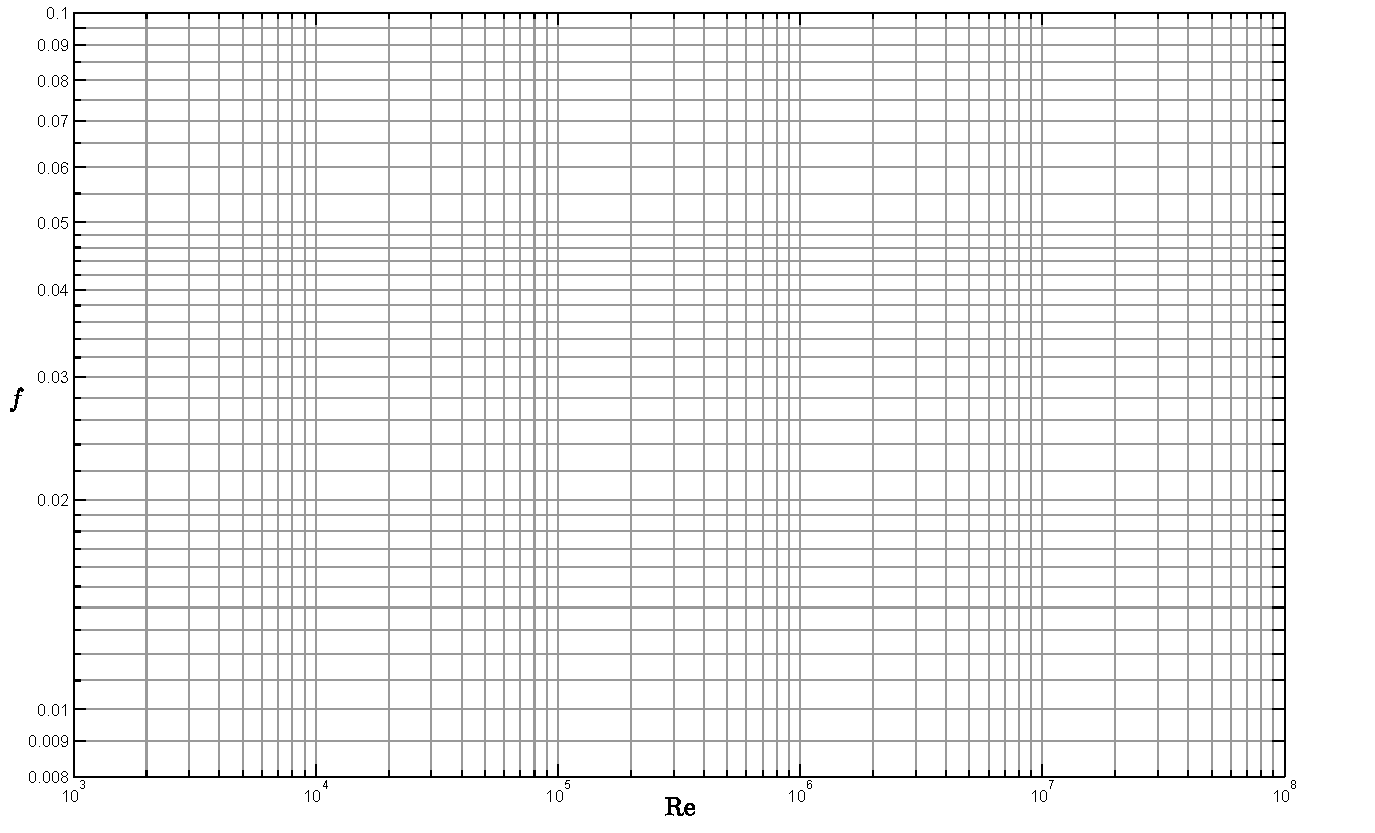
\includegraphics[width=\textwidth]{../fig/stroming_in_leidingen/Moody_diagram_empirisch_leeg}
		}
		\only<2>{
			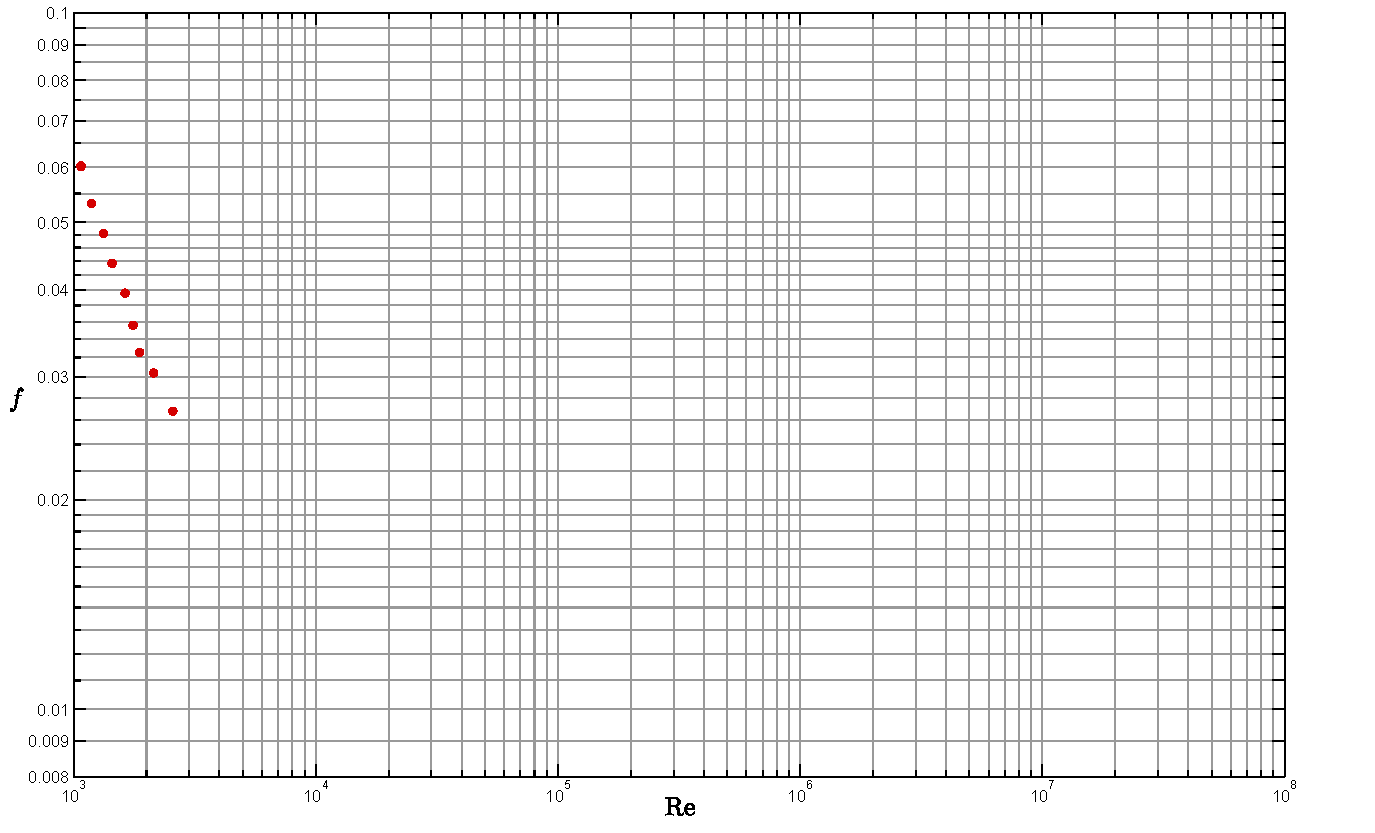
\includegraphics[width=\textwidth]{../fig/stroming_in_leidingen/Moody_diagram_empirisch0_laminair}
		}
		\only<3>{
			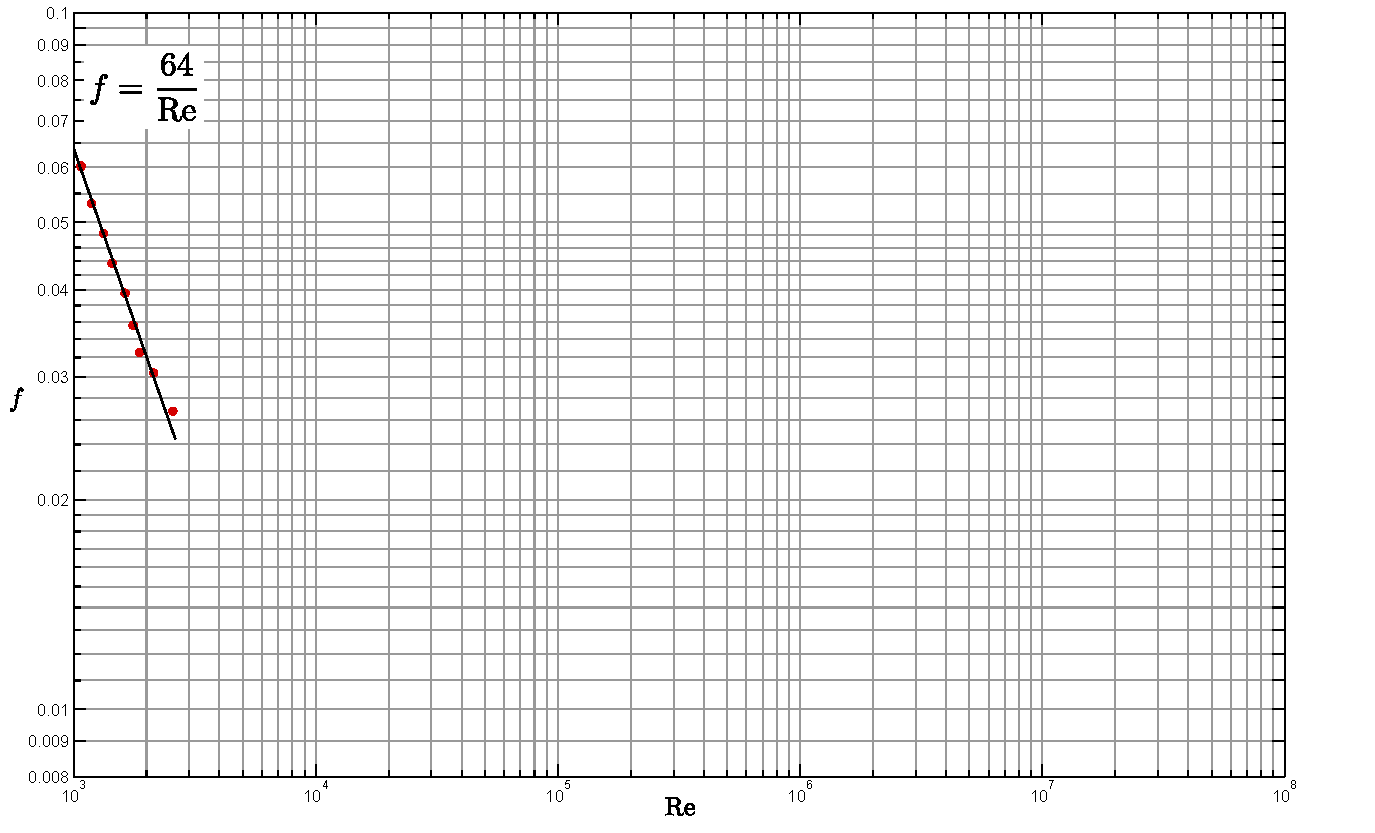
\includegraphics[width=\textwidth]{../fig/stroming_in_leidingen/Moody_diagram_empirisch0_laminair_fit}
		}
		\only<4>{
			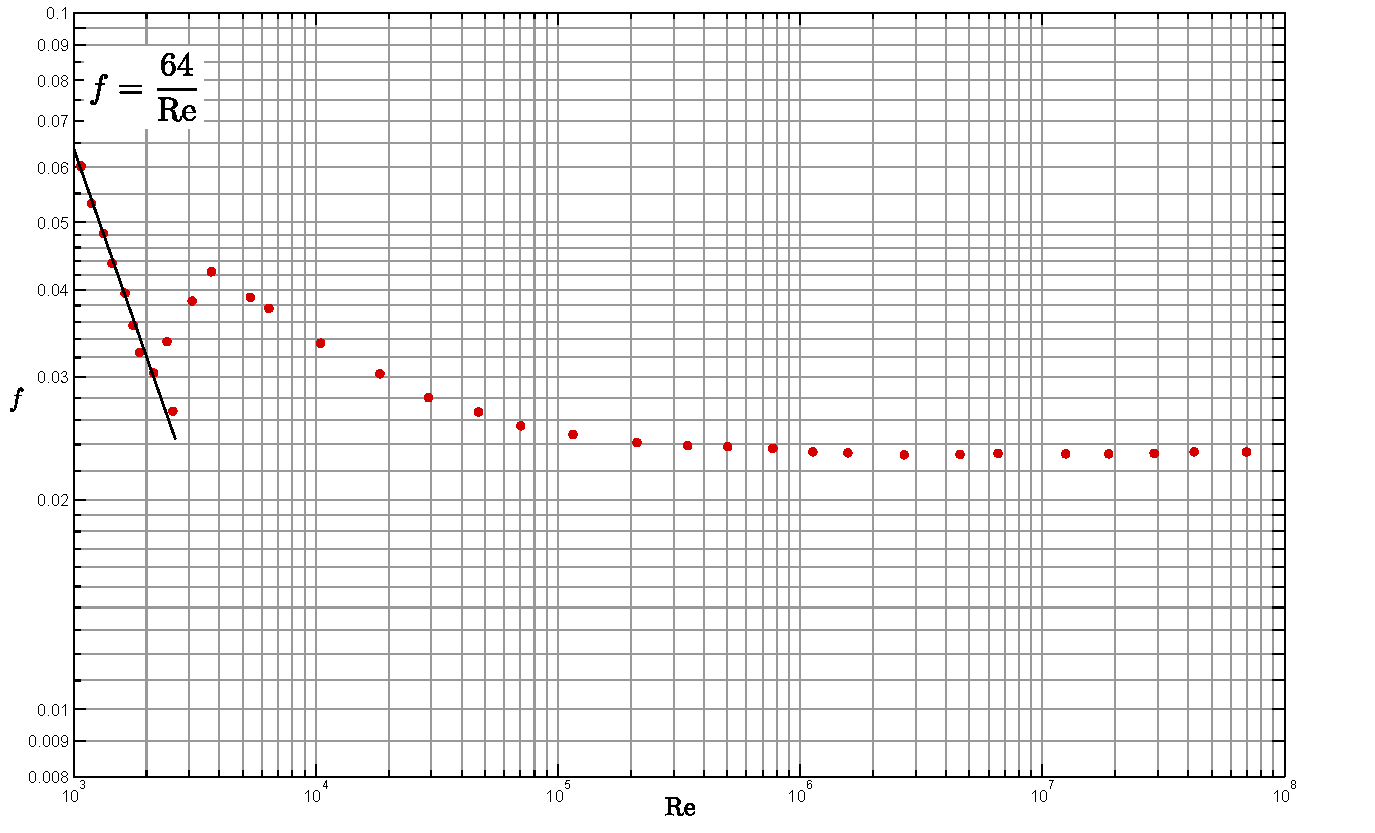
\includegraphics[width=\textwidth]{../fig/stroming_in_leidingen/Moody_diagram_empirisch0}
		}
		\only<5>{
			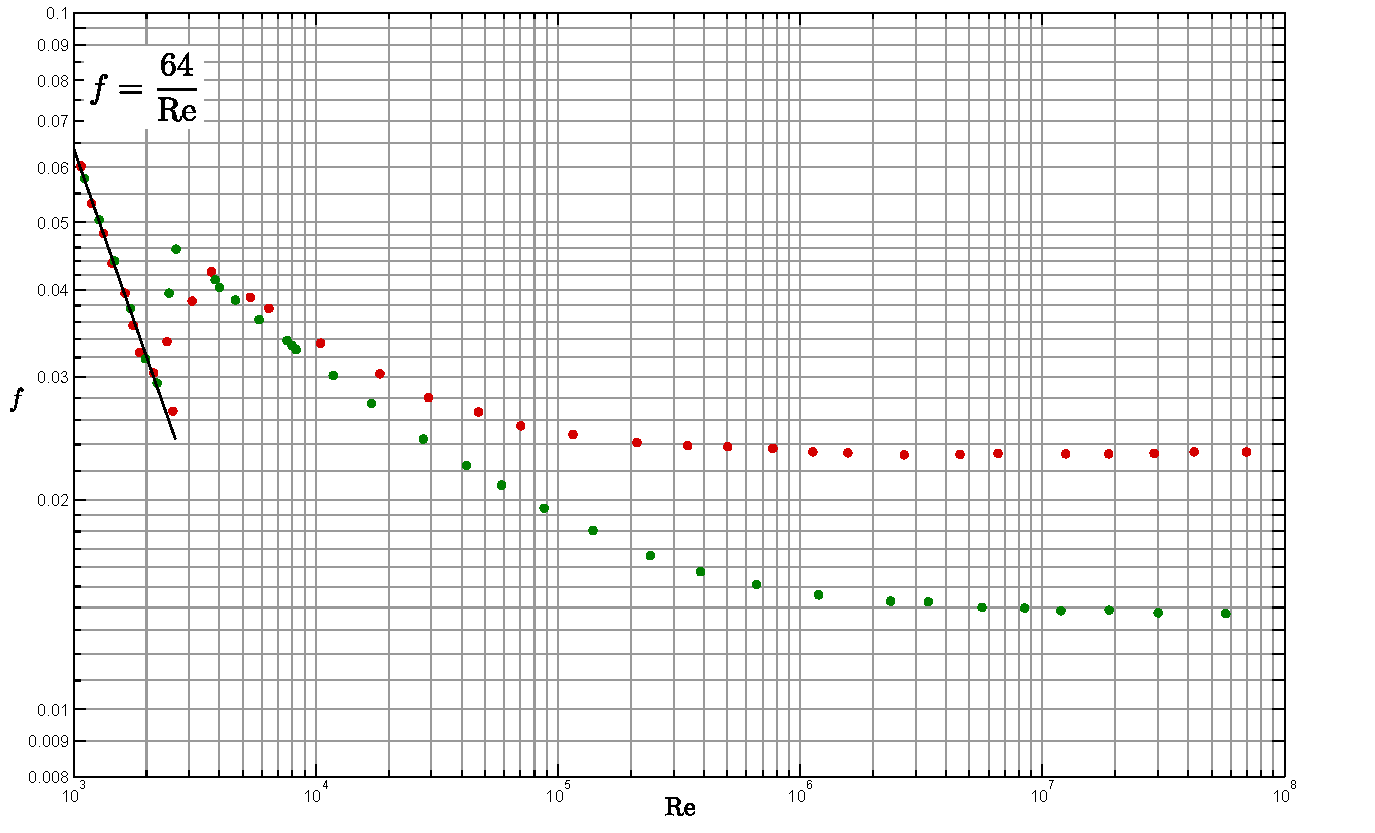
\includegraphics[width=\textwidth]{../fig/stroming_in_leidingen/Moody_diagram_empirisch1}
		}
		\only<6>{
			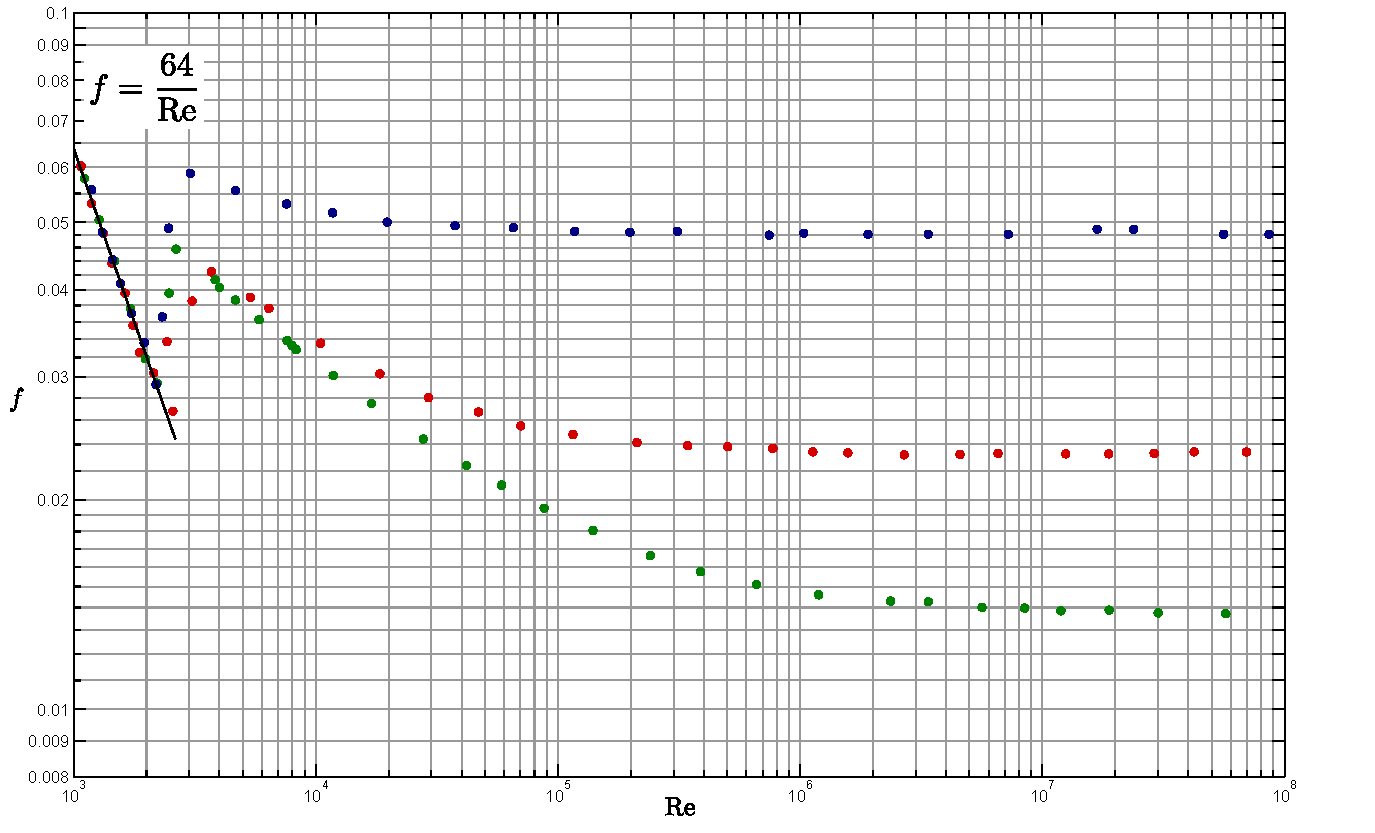
\includegraphics[width=\textwidth]{../fig/stroming_in_leidingen/Moody_diagram_empirisch2}
		}
		\only<7>{
			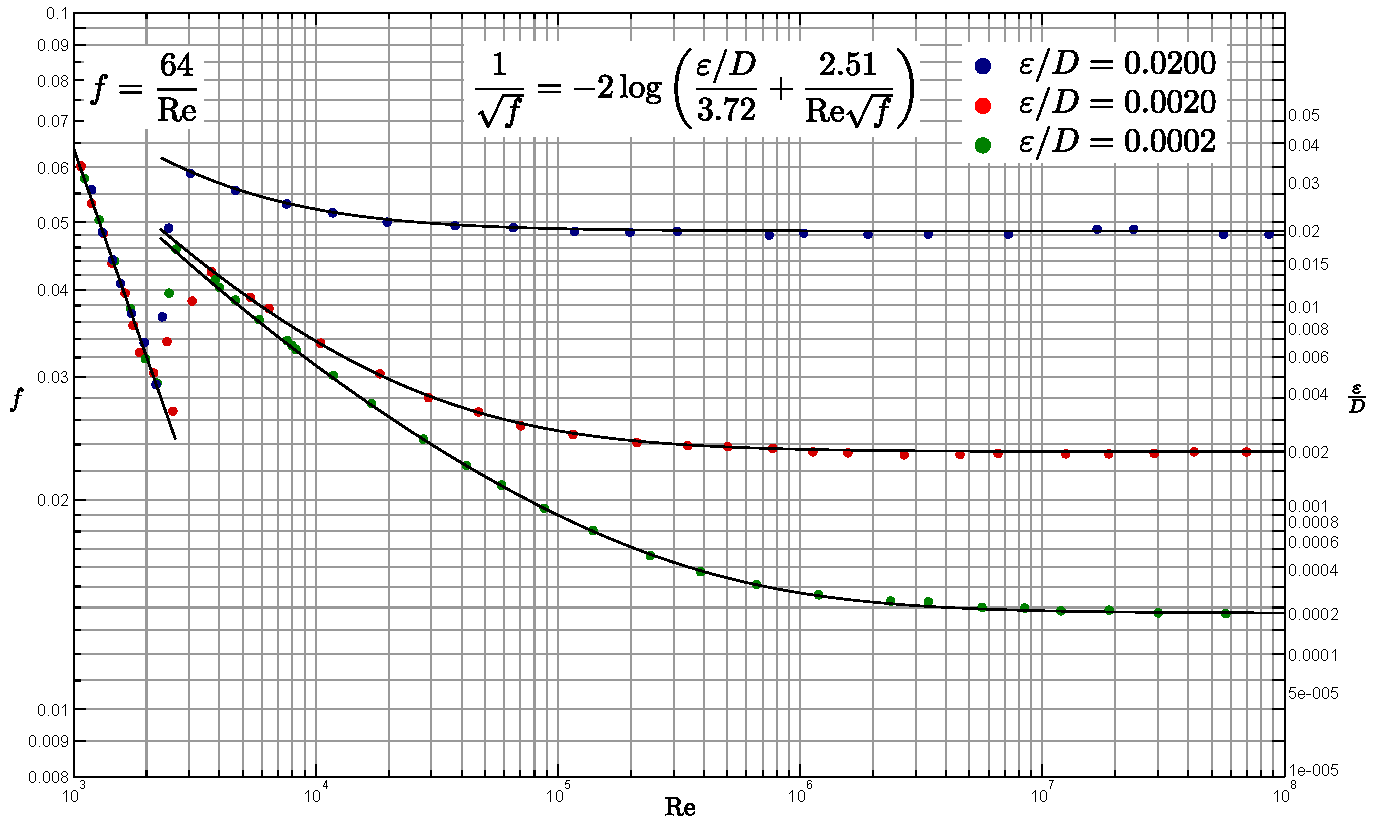
\includegraphics[width=\textwidth]{../fig/stroming_in_leidingen/Moody_diagram_empirisch_turbulent_fit}
		}
		\only<8>{
			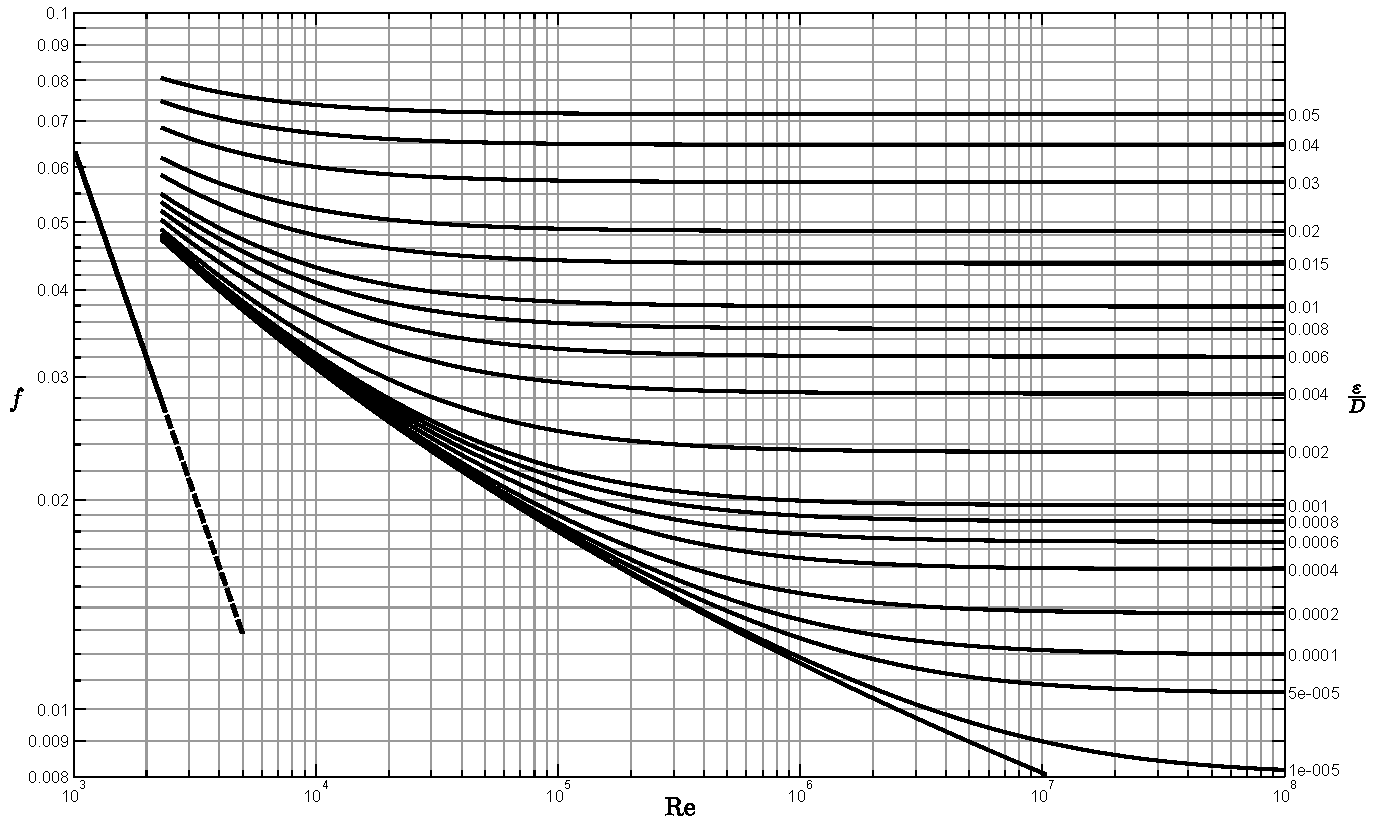
\includegraphics[width=\textwidth]{../fig/stroming_in_leidingen/Moody_diagram}
		}
	\end{frame}
%%%%%%%%%%%%%%%%%%%%%%%%%%%%%%%%%%%%%%%%%%%%%%%%%%%%%%%%%%%%%%%%%%%%%%%%%%%
  	\begin{frame}
		\frametitle{Dimensieanalyse}
		\vspace{1cm}
		\begin{equation*}
			\Delta p = \phi(L,D,v,\mu,\rho,\varepsilon)
		\end{equation*}
		\vspace{0.5cm}
		\begin{equation*}
			\Delta p = f(Re,\varepsilon/D) \frac{1}{2}\rho v^2 \frac{L}{D}
		\end{equation*}
		\pause
		\center
		De wrijvingsfactor $f$ voor turbulente stroming moet bepaald worden met behulp van empirische data:
		
		Moody diagram
	\end{frame}
%%%%%%%%%%%%%%%%%%%%%%%%%%%%%%%%%%%%%%%%%%%%%%%%%%%%%%%%%%%%%%%%%%%%%%%%%%%
  	\begin{frame}
		\frametitle{Moody diagram}
		\center
		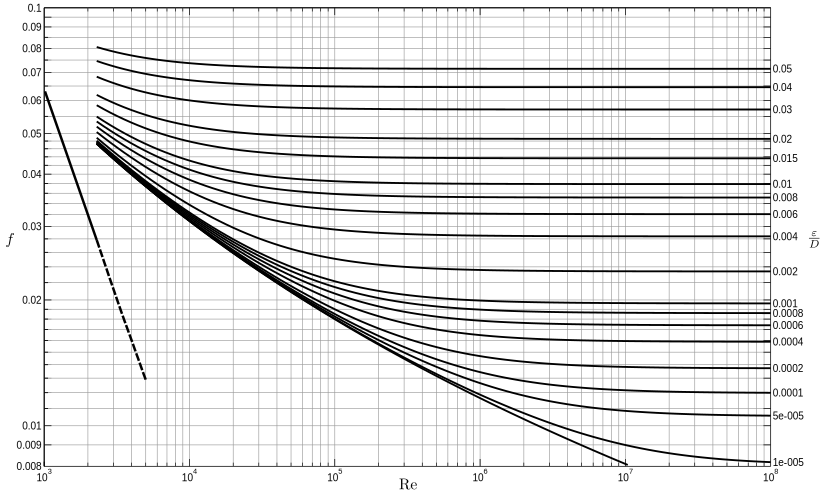
\includegraphics[width=\textwidth]{../fig/stroming_in_leidingen/Moody_diagram_regimes}
	\end{frame}
%%%%%%%%%%%%%%%%%%%%%%%%%%%%%%%%%%%%%%%%%%%%%%%%%%%%%%%%%%%%%%%%%%%%%%%%%%%
  	\begin{frame}
		\frametitle{Gebruik van het Moody diagram}
		\center
		\only<1>{
			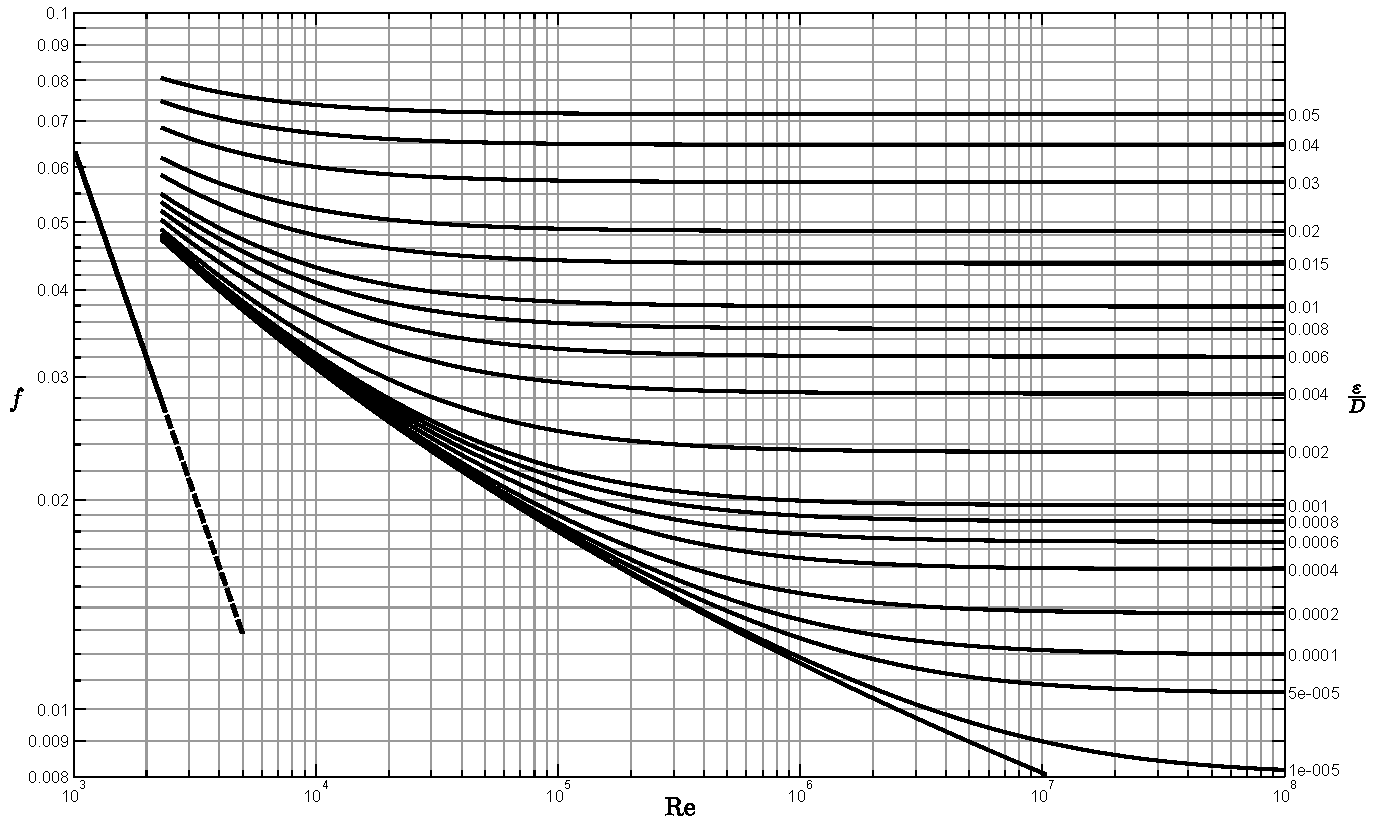
\includegraphics[width=\textwidth]{../fig/stroming_in_leidingen/Moody_diagram_gebruik}
		}
		\only<2>{
			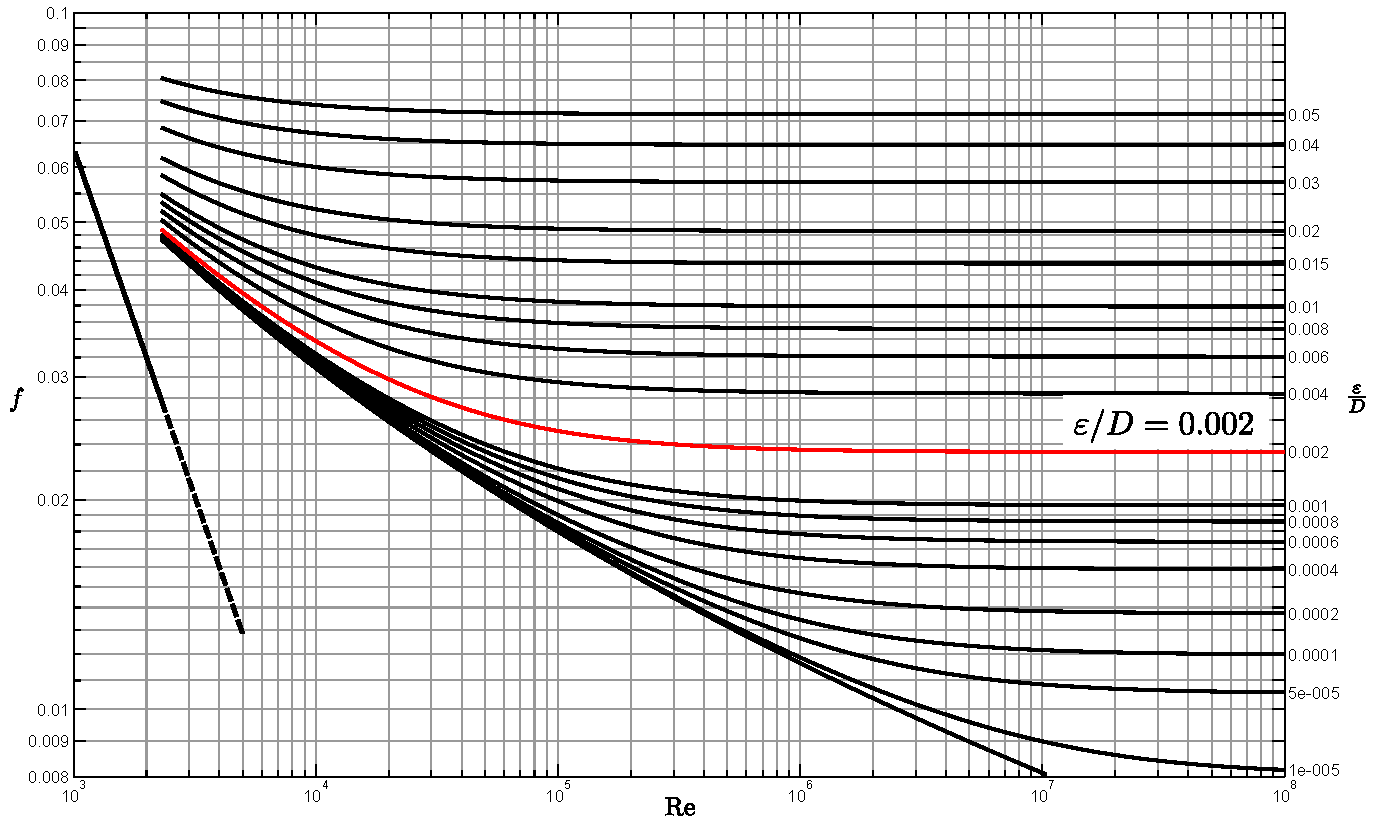
\includegraphics[width=\textwidth]{../fig/stroming_in_leidingen/Moody_diagram_gebruik1}
		}
		\only<3>{
			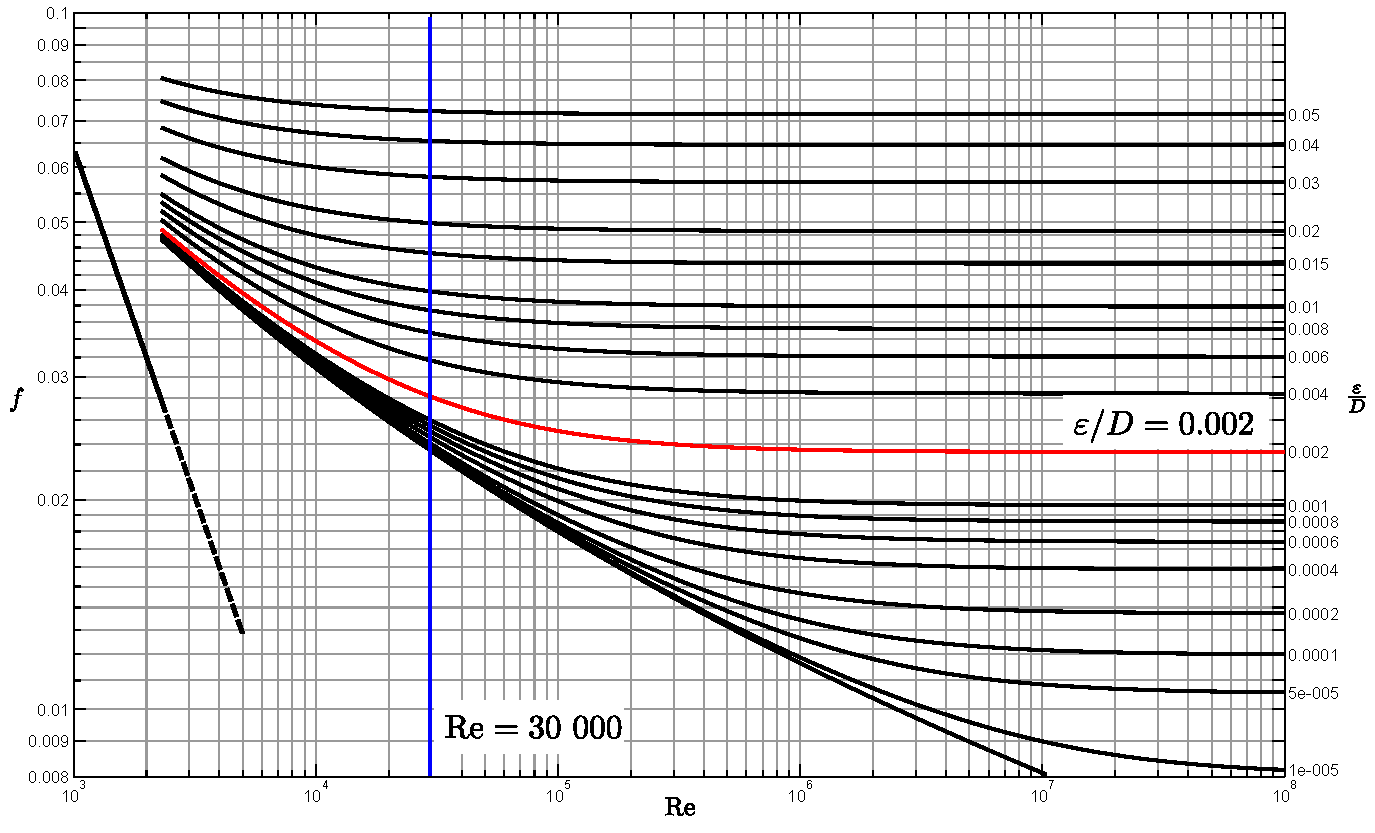
\includegraphics[width=\textwidth]{../fig/stroming_in_leidingen/Moody_diagram_gebruik2}
		}
		\only<4>{
			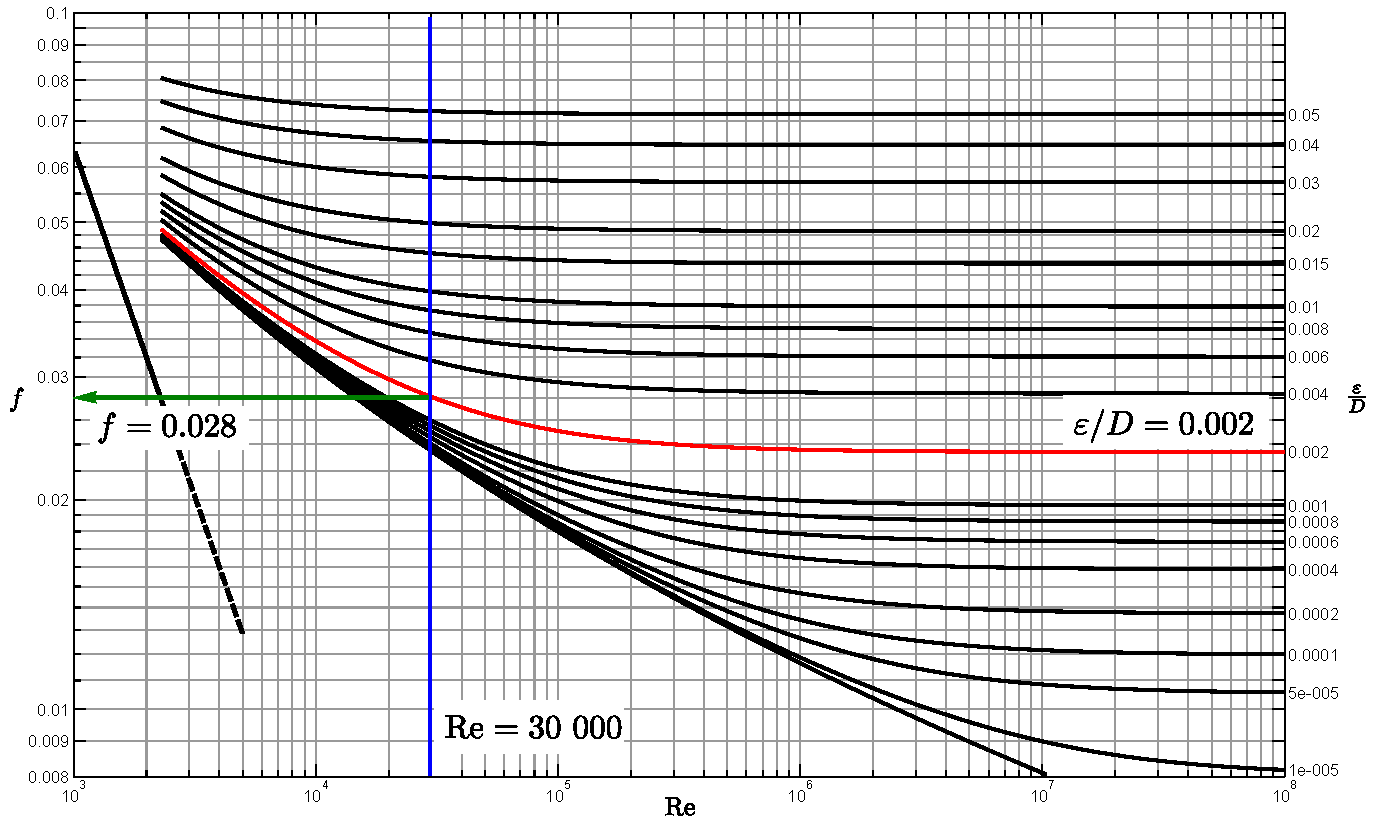
\includegraphics[width=\textwidth]{../fig/stroming_in_leidingen/Moody_diagram_gebruik3}
		}
	\end{frame}
%%%%%%%%%%%%%%%%%%%%%%%%%%%%%%%%%%%%%%%%%%%%%%%%%%%%%%%%%%%%%%%%%%%%%%%%%%%
  	\begin{frame}
		\frametitle{Turbulent snelheidsprofiel}
		\vspace{0.5cm}
		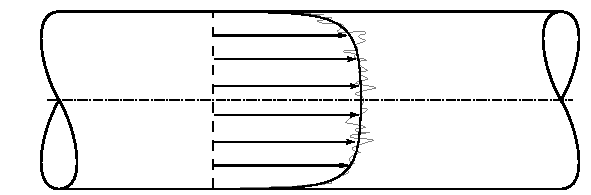
\includegraphics[width=\textwidth]{../fig/stroming_in_leidingen/Turbulent_snelheidsprofiel}
		\pause
		\vspace{0.5cm}
		\begin{equation*}
			\frac{\bar{v}}{v_{\text{max}}} \approx \left(1- \frac{r}{R}\right)^{1/7}
		\end{equation*}
	\end{frame}
%%%%%%%%%%%%%%%%%%%%%%%%%%%%%%%%%%%%%%%%%%%%%%%%%%%%%%%%%%%%%%%%%%%%%%%%%%%
  	\begin{frame}
		\frametitle{Invloed van ruwheid}
		\vspace{1cm}
		\center
		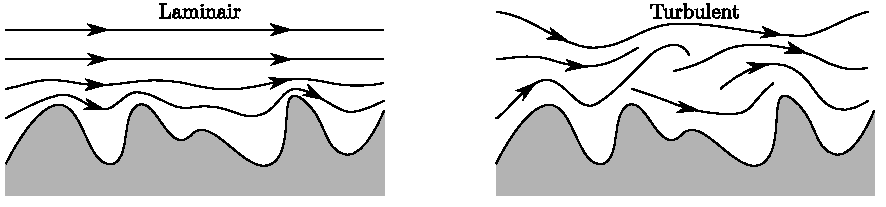
\includegraphics[width=\textwidth]{../fig/stroming_in_leidingen/Ruwheid_laminair_turbulent}
		
		\pause
		\vspace{0.5cm}
		Bij laminaire stroming worden door de ruwheid geïnduceerde fluctuaties door de viskeuze krachten afgevlakt
		
		\pause
		\vspace{0.5cm}
		Bij turbulente stroming hebben door de ruwheid geïnduceerde fluctuaties invloed in de volledige stroming
	\end{frame}
%%%%%%%%%%%%%%%%%%%%%%%%%%%%%%%%%%%%%%%%%%%%%%%%%%%%%%%%%%%%%%%%%%%%%%%%%%%
\end{document}